\documentclass[paper=letter,11pt]{scrartcl}

\KOMAoptions{headinclude=true, footinclude=false}
\KOMAoptions{DIV=14, BCOR=5mm}
\KOMAoptions{numbers=noendperiod}
\KOMAoptions{parskip=half}
\addtokomafont{disposition}{\rmfamily}
\addtokomafont{part}{\LARGE}
\addtokomafont{descriptionlabel}{\rmfamily}
%\setkomafont{pageheadfoot}{\normalsize\sffamily}
\setkomafont{pagehead}{\normalsize\rmfamily}
%\setkomafont{publishers}{\normalsize\rmfamily}
\setkomafont{caption}{\normalfont\small}
\setcapindent{0pt}
\deffootnote[1em]{1em}{1em}{\textsuperscript{\thefootnotemark}\ }


\usepackage{amsmath}
\usepackage[varg]{txfonts}
\usepackage[T1]{fontenc}
\usepackage{graphicx}
\usepackage{xcolor}
\usepackage[american]{babel}
% hyperref is needed in many places, so include it here
\usepackage{hyperref}

\usepackage{xspace}
\usepackage{multirow}
\usepackage{float}


\usepackage{braket}
\usepackage{bbm}
\usepackage{relsize}
\usepackage{tcolorbox}

\def\ketY{\ensuremath{\ket {\Psi}}}
\def\iGeV{\ensuremath{\textrm{GeV}^{-1}}}
%\def\mp{\ensuremath{m_{\textrm{proton}}}}
\def\rp{\ensuremath{r_{\textrm{proton}}}}
\def\me{\ensuremath{m_{\textrm{electron}}}}
\def\aG{\ensuremath{\alpha_G}}
\def\rAtom{\ensuremath{r_{\textrm{atom}}}}
\def\rNucl{\ensuremath{r_{\textrm{nucleus}}}}
\def\GN{\ensuremath{\textrm{G}_\textrm{N}}}
\def\ketX{\ensuremath{\ket{\vec{x}}}}
\def\ve{\ensuremath{\vec{\epsilon}}}


\def\ABCDMatrix{\ensuremath{\begin{pmatrix} A &  B  \\ C  & D \end{pmatrix}}}
\def\xyprime{\ensuremath{\begin{pmatrix} x' \\ y' \end{pmatrix}}}
\def\xyprimeT{\ensuremath{\begin{pmatrix} x' &  y' \end{pmatrix}}}
\def\xy{\ensuremath{\begin{pmatrix} x \\ y \end{pmatrix}}}
\def\xyT{\ensuremath{\begin{pmatrix} x & y \end{pmatrix}}}

\def\IMatrix{\ensuremath{\begin{pmatrix} 0 &  1  \\ -1  & 0 \end{pmatrix}}}
\def\IBoostMatrix{\ensuremath{\begin{pmatrix} 0 &  1  \\ 1  & 0 \end{pmatrix}}}
\def\JThree{\ensuremath{\begin{pmatrix}    0 & -i & 0  \\ i & 0  & 0 \\ 0 & 0 & 0 \end{pmatrix}}} 
\def\JTwo{\ensuremath{\begin{bmatrix}    0 & 0 & -i  \\ 0 & 0  & 0 \\ i & 0 & 0 \end{bmatrix}}}
\def\JOne{\ensuremath{\begin{bmatrix}    0 & 0 & 0  \\ 0 & 0  & -i \\ 0 & i & 0 \end{bmatrix}}}
\def\etamn{\ensuremath{\eta_{\mu\nu}}}
\def\Lmn{\ensuremath{\Lambda^\mu_\nu}}
\def\dmn{\ensuremath{\delta^\mu_\nu}}
\def\wmn{\ensuremath{\omega^\mu_\nu}}
\def\be{\begin{equation*}}
\def\ee{\end{equation*}}
\def\bea{\begin{eqnarray*}}
\def\eea{\end{eqnarray*}}
\def\bi{\begin{itemize}}
\def\ei{\end{itemize}}
\def\fmn{\ensuremath{F_{\mu\nu}}}
\def\fMN{\ensuremath{F^{\mu\nu}}}
\def\bc{\begin{center}}
\def\ec{\end{center}}
\def\nus{$\nu$s}

\def\adagger{\ensuremath{a_{p\sigma}^\dagger}}
\def\lineacross{\noindent\rule{\textwidth}{1pt}}

\newcommand{\multiline}[1] {
\begin{tabular} {|l}
#1
\end{tabular}
}

\newcommand{\multilineNoLine}[1] {
\begin{tabular} {l}
#1
\end{tabular}
}



\newcommand{\lineTwo}[2] {
\begin{tabular} {|l}
#1 \\
#2
\end{tabular}
}

\newcommand{\rmt}[1] {
\textrm{#1}
}


%
% Units
%
\def\m{\ensuremath{\rmt{m}}}
\def\GeV{\ensuremath{\rmt{GeV}}}
\def\pt{\ensuremath{p_\rmt{T}}}


\def\parity{\ensuremath{\mathcal{P}}}

\usepackage{cancel}
\usepackage{ mathrsfs }
\def\bigL{\ensuremath{\mathscr{L}}}

\usepackage{ dsfont }



\usepackage{fancyhdr}
\fancyhf{}

%\documentclass[margin,line]{res}
\usepackage{braket}
\usepackage{bbm}
\usepackage{relsize}
\usepackage{tcolorbox}


\def\ketY{\ensuremath{\ket {\Psi}}}
\def\iGeV{\ensuremath{\textrm{GeV}^{-1}}}
%\def\mp{\ensuremath{m_{\textrm{proton}}}}
\def\rp{\ensuremath{r_{\textrm{proton}}}}
\def\me{\ensuremath{m_{\textrm{electron}}}}
\def\aG{\ensuremath{\alpha_G}}
\def\rAtom{\ensuremath{r_{\textrm{atom}}}}
\def\rNucl{\ensuremath{r_{\textrm{nucleus}}}}
\def\GN{\ensuremath{\textrm{G}_\textrm{N}}}
\def\ketX{\ensuremath{\ket{\vec{x}}}}
\def\ve{\ensuremath{\vec{\epsilon}}}


\def\ABCDMatrix{\ensuremath{\begin{pmatrix} A &  B  \\ C  & D \end{pmatrix}}}
\def\xyprime{\ensuremath{\begin{pmatrix} x' \\ y' \end{pmatrix}}}
\def\xyprimeT{\ensuremath{\begin{pmatrix} x' &  y' \end{pmatrix}}}
\def\xy{\ensuremath{\begin{pmatrix} x \\ y \end{pmatrix}}}
\def\xyT{\ensuremath{\begin{pmatrix} x & y \end{pmatrix}}}

\def\IMatrix{\ensuremath{\begin{pmatrix} 0 &  1  \\ -1  & 0 \end{pmatrix}}}
\def\IBoostMatrix{\ensuremath{\begin{pmatrix} 0 &  1  \\ 1  & 0 \end{pmatrix}}}
\def\JThree{\ensuremath{\begin{pmatrix}    0 & -i & 0  \\ i & 0  & 0 \\ 0 & 0 & 0 \end{pmatrix}}} 
\def\JTwo{\ensuremath{\begin{bmatrix}    0 & 0 & -i  \\ 0 & 0  & 0 \\ i & 0 & 0 \end{bmatrix}}}
\def\JOne{\ensuremath{\begin{bmatrix}    0 & 0 & 0  \\ 0 & 0  & -i \\ 0 & i & 0 \end{bmatrix}}}
\def\etamn{\ensuremath{\eta_{\mu\nu}}}
\def\Lmn{\ensuremath{\Lambda^\mu_\nu}}
\def\dmn{\ensuremath{\delta^\mu_\nu}}
\def\wmn{\ensuremath{\omega^\mu_\nu}}
\def\be{\begin{equation*}}
\def\ee{\end{equation*}}
\def\bea{\begin{eqnarray*}}
\def\eea{\end{eqnarray*}}
\def\bi{\begin{itemize}}
\def\ei{\end{itemize}}
\def\fmn{\ensuremath{F_{\mu\nu}}}
\def\fMN{\ensuremath{F^{\mu\nu}}}
\def\bc{\begin{center}}
\def\ec{\end{center}}
\def\nus{$\nu$s}

\def\adagger{\ensuremath{a_{p\sigma}^\dagger}}
\def\lineacross{\noindent\rule{\textwidth}{1pt}}

\newcommand{\multiline}[1] {
\begin{tabular} {|l}
#1
\end{tabular}
}

\newcommand{\multilineNoLine}[1] {
\begin{tabular} {l}
#1
\end{tabular}
}



\newcommand{\lineTwo}[2] {
\begin{tabular} {|l}
#1 \\
#2
\end{tabular}
}

\newcommand{\rmt}[1] {
\textrm{#1}
}


%
% Units
%
\def\m{\ensuremath{\rmt{m}}}
\def\GeV{\ensuremath{\rmt{GeV}}}
\def\pt{\ensuremath{p_\rmt{T}}}


\def\parity{\ensuremath{\mathcal{P}}}

\usepackage{cancel}
\usepackage{ mathrsfs }
\def\bigL{\ensuremath{\mathscr{L}}}

\usepackage{ dsfont }


\usepackage{cancel}

\usepackage{fancyhdr}

\fancyhf{}
\lhead{\Large 33-444} % \hfill Introduction to Particle Physics \hfill Spring 2020}
\chead{\Large Introduction to Particle Physics} % \hfill Spring 2020}
\rhead{\Large Spring 2020} % \hfill Introduction to Particle Physics \hfill Spring 2020}

\begin{document}
\thispagestyle{fancy}

\begin{center}
{\huge \textbf{Lecture 17}}
\end{center}

{\fontsize{14}{16}\selectfont

\underline{Lorentz Invariance and ``Soft Limits''}

Punch line that we've been building to in first part of this course.

Matrix element we would get by scattering external $\gamma$.


\be
M = \epsilon^\mu M_\mu
\ee
where $\epsilon^\mu$ is some linear combination of two photon polarization vector $\epsilon^1$ and $\epsilon^2$


M is Lorentz Invariant, under lorentz transformation
\be
M \rightarrow \epsilon'^\mu M'_\mu
\ee
where $M'_\mu = {\Lambda_\mu}^\nu M_\nu$

However (here comes the major constraint) $\epsilon$ is not  a full 4-vector.  
Only has 2 components.

Under little group transformations (you will show in your H.W.)
\be
\epsilon \rightarrow \underbrace{c_1 \epsilon_1^\mu + c_2 \epsilon_2^\mu}_{\substack{\epsilon' \textrm{ can only be made} \\ \textrm{ of these pieces}}} + \underbrace{c_3 p^\mu}_{\substack{\textrm{Not valid} \\ \textrm{``Not in Hilbert Space''}}}
\ee


So, 
\bea
M=\epsilon^\mu M_\mu &\rightarrow& \left(c_1 \epsilon_1^\mu + c_2 \epsilon_2^\mu + c_3 p^\mu \right) M'_\mu \\
&=& \epsilon'^\mu M'_\mu + \underbrace{c_3 p^\mu M'_\mu}_{\textrm{Must go to 0}}
\eea

We will see, this has enourmous implications !!!

\clearpage


Will be considering diagrams with external ``$\gamma$''s (massless spin 1 particles)

\begin{figure}[h]
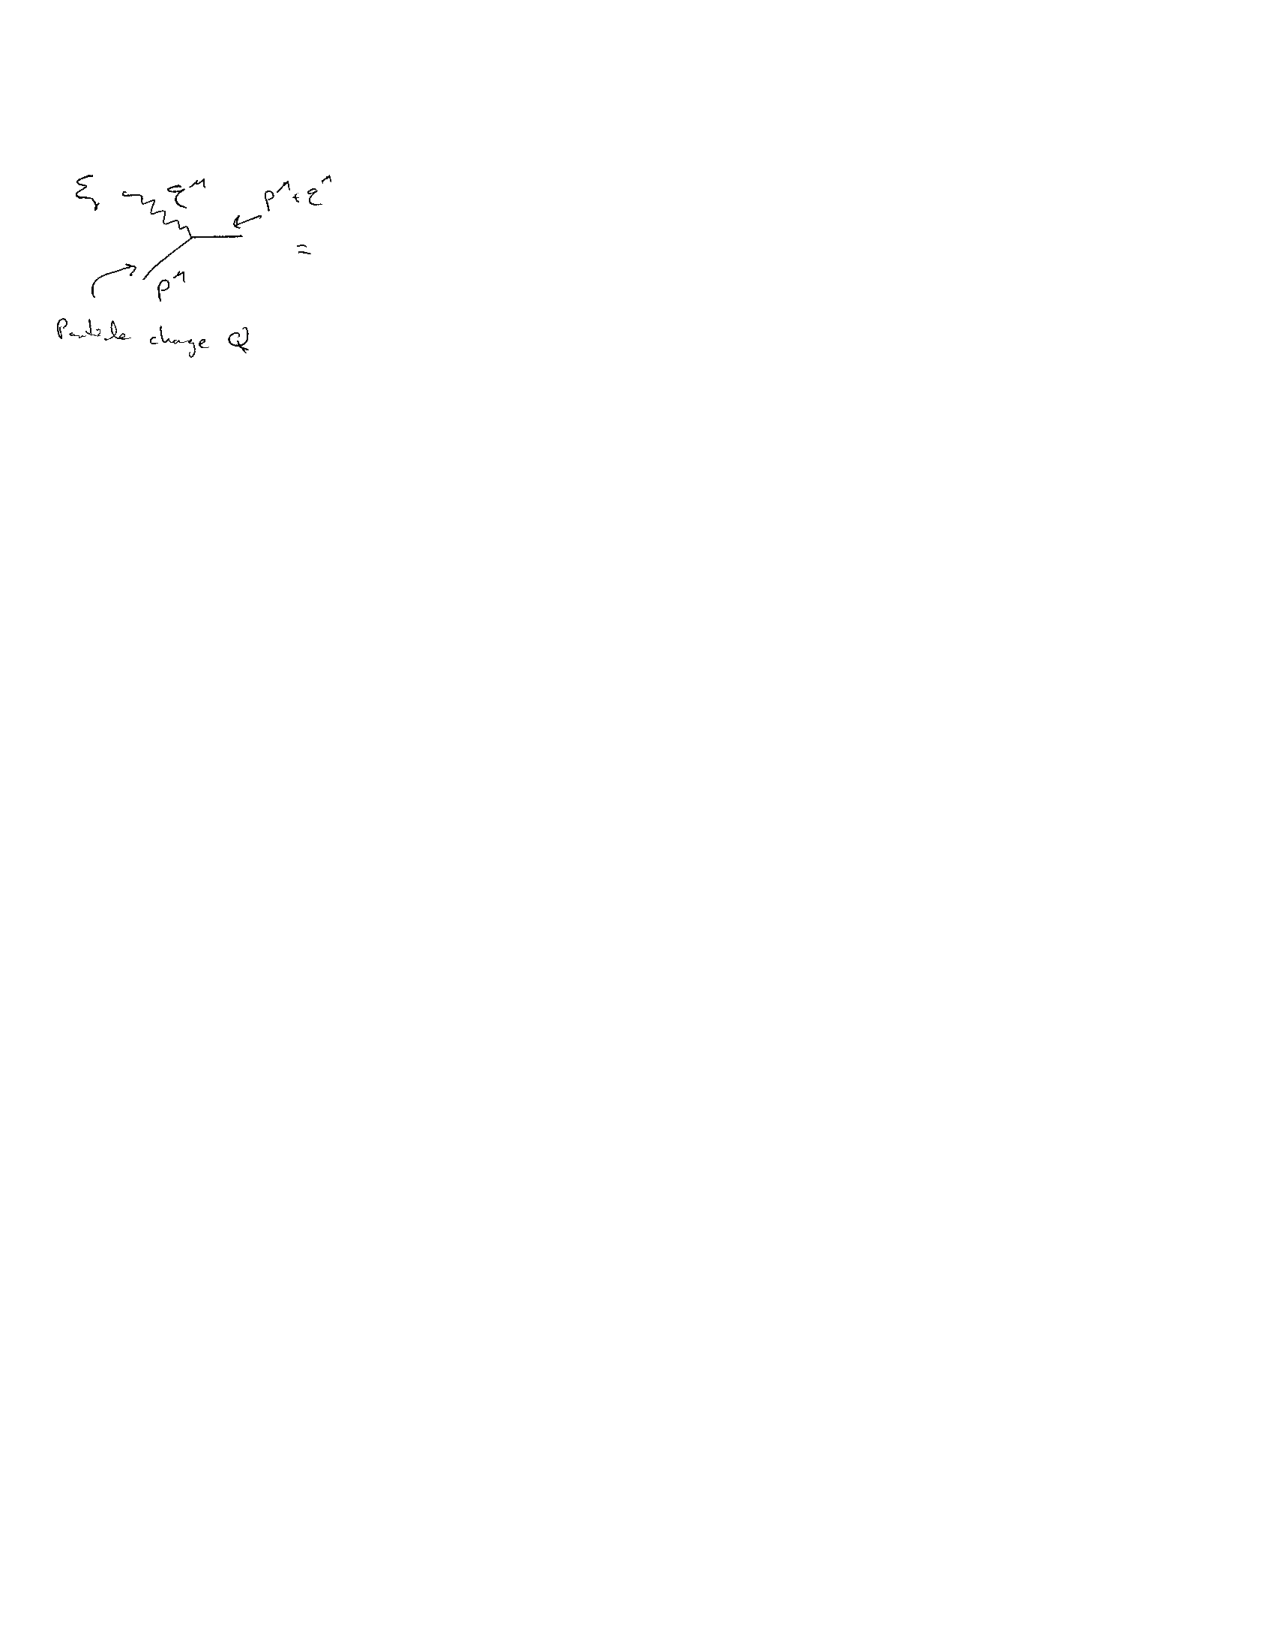
\includegraphics[width=0.5\textwidth]{./gammaVertex.pdf}
\end{figure}
\bea
&=& iQ(p^\mu + (p^\mu + q^\mu)) \epsilon_\mu    \hspace*{1in} (q^\mu\epsilon_\mu = 0) \\
&=& iQ 2 p^\mu \epsilon_\mu
\eea


This is the most general form in the ``soft limit''  $q\rightarrow0$

\fbox{\begin{minipage}{0.6\textwidth}
\be
\Gamma_\mu \sim p_\mu F(q^2, p^2, p\cdot q) 
\ee
By dimensional analyiss $F(q^2, p^2, p\cdot q) \rightarrow F(\frac{p\cdot q}{m^2})$
\end{minipage}}

\lineacross

\clearpage

Consider ``Compton Scattering''


Start with one type of spin-1 boson and one type of matter particle.

The diagram: 
\begin{figure}[h]
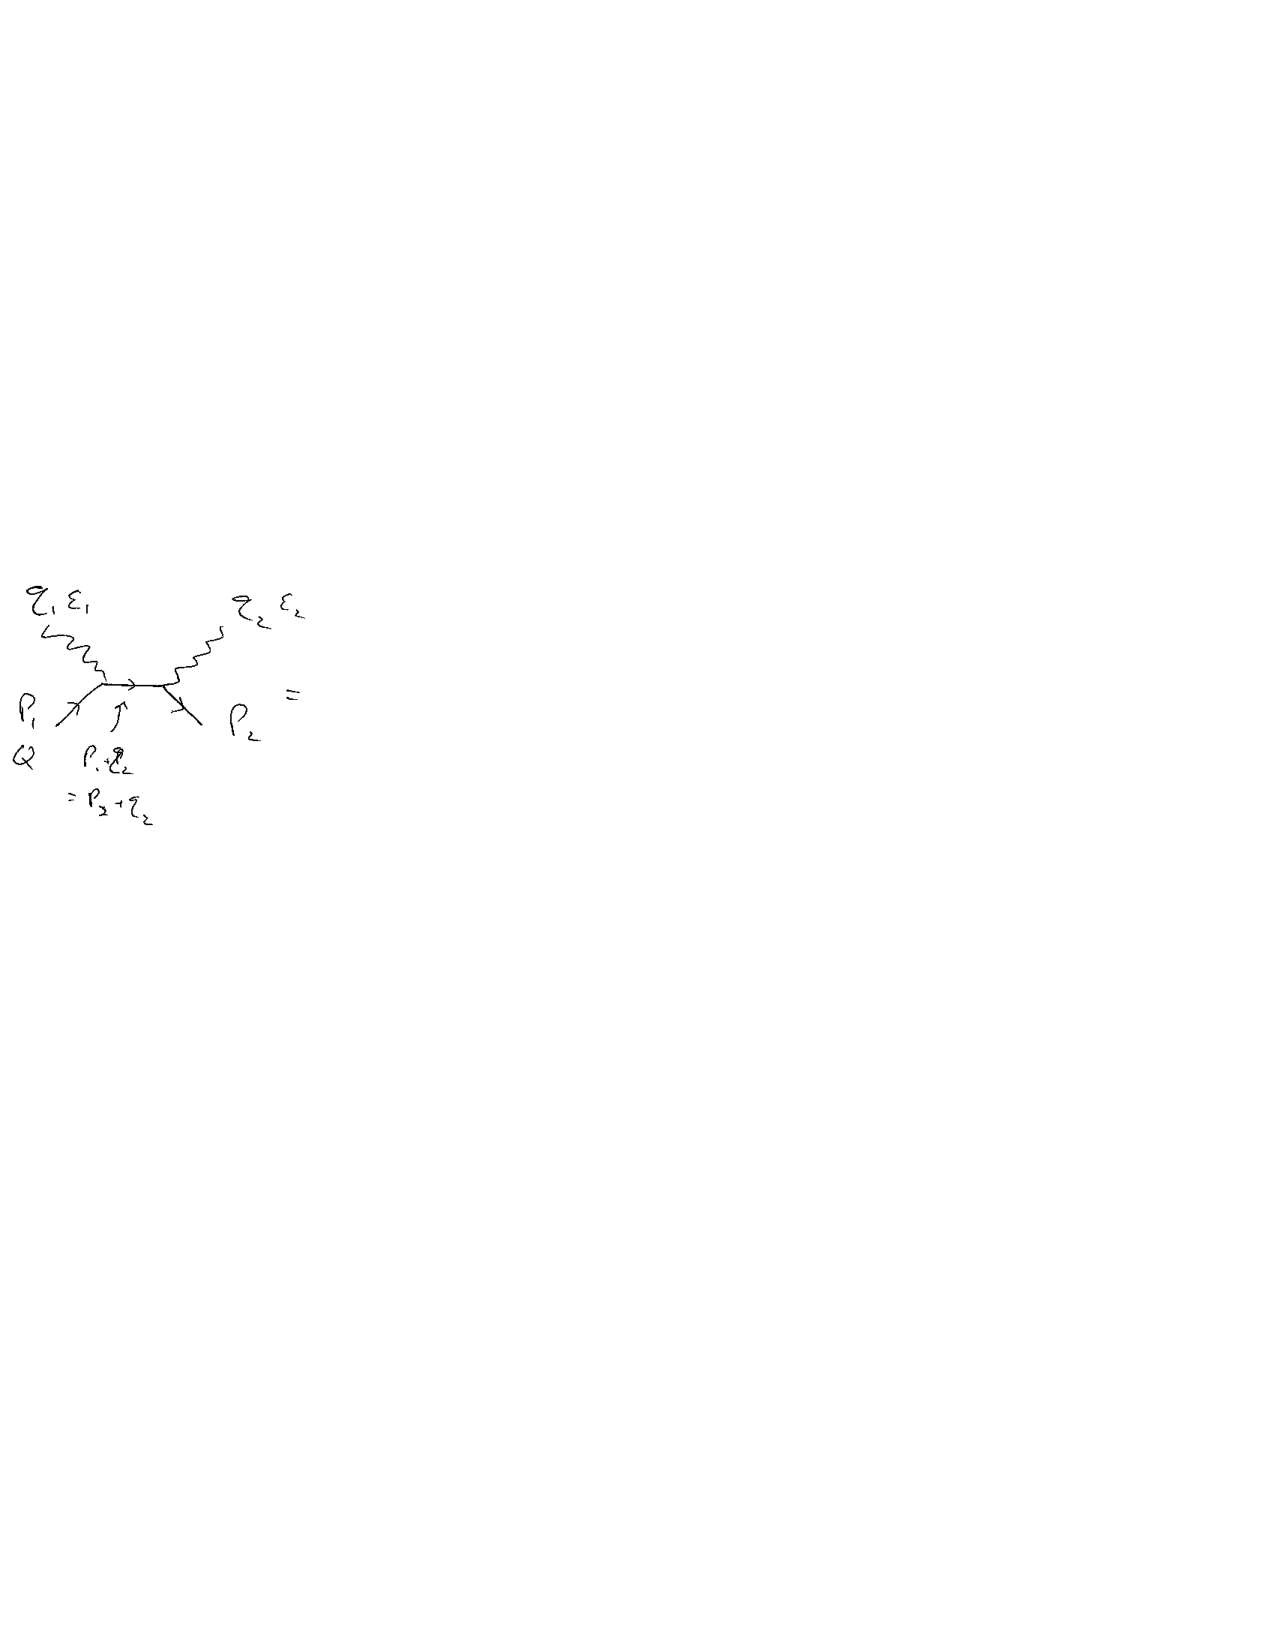
\includegraphics[width=0.5\textwidth]{./comptonScattering.pdf}
\end{figure}
\bea
&=& (iQ)\epsilon^1_\mu(2 p_1^\mu) \frac{i}{(p_1+q_1)^2 - m^2} (iQ)\epsilon^2_\nu (2p_2^\nu)\\
&=& (-iQ^2) 4 \frac{(p_1\cdot\epsilon^1) (p_2\cdot\epsilon^2)}{m^2 + 2 p_1\cdot q_1 -m^2 }  = \epsilon_1^\mu \epsilon_2^\nu \underbrace{\left( \frac{(-iQ^2) 2 {p_1}_\mu {p_2}_\nu}{p_1\cdot q_1} \right)}_{M_{\mu\nu}}
\eea

As we said above, Lorentz Invariant $\Rightarrow q_1^\mu q_2^\nu M_{\mu\nu} = 0$\\

But here, $ q_1^\mu q_2^\nu M_{\mu\nu} = (-iQ^2) 2 (p_2\cdot q_2) \ne 0$ !

Looks like we're dead...

\lineacross

\clearpage

However we are forgetting a diagram.

\begin{figure}[h]
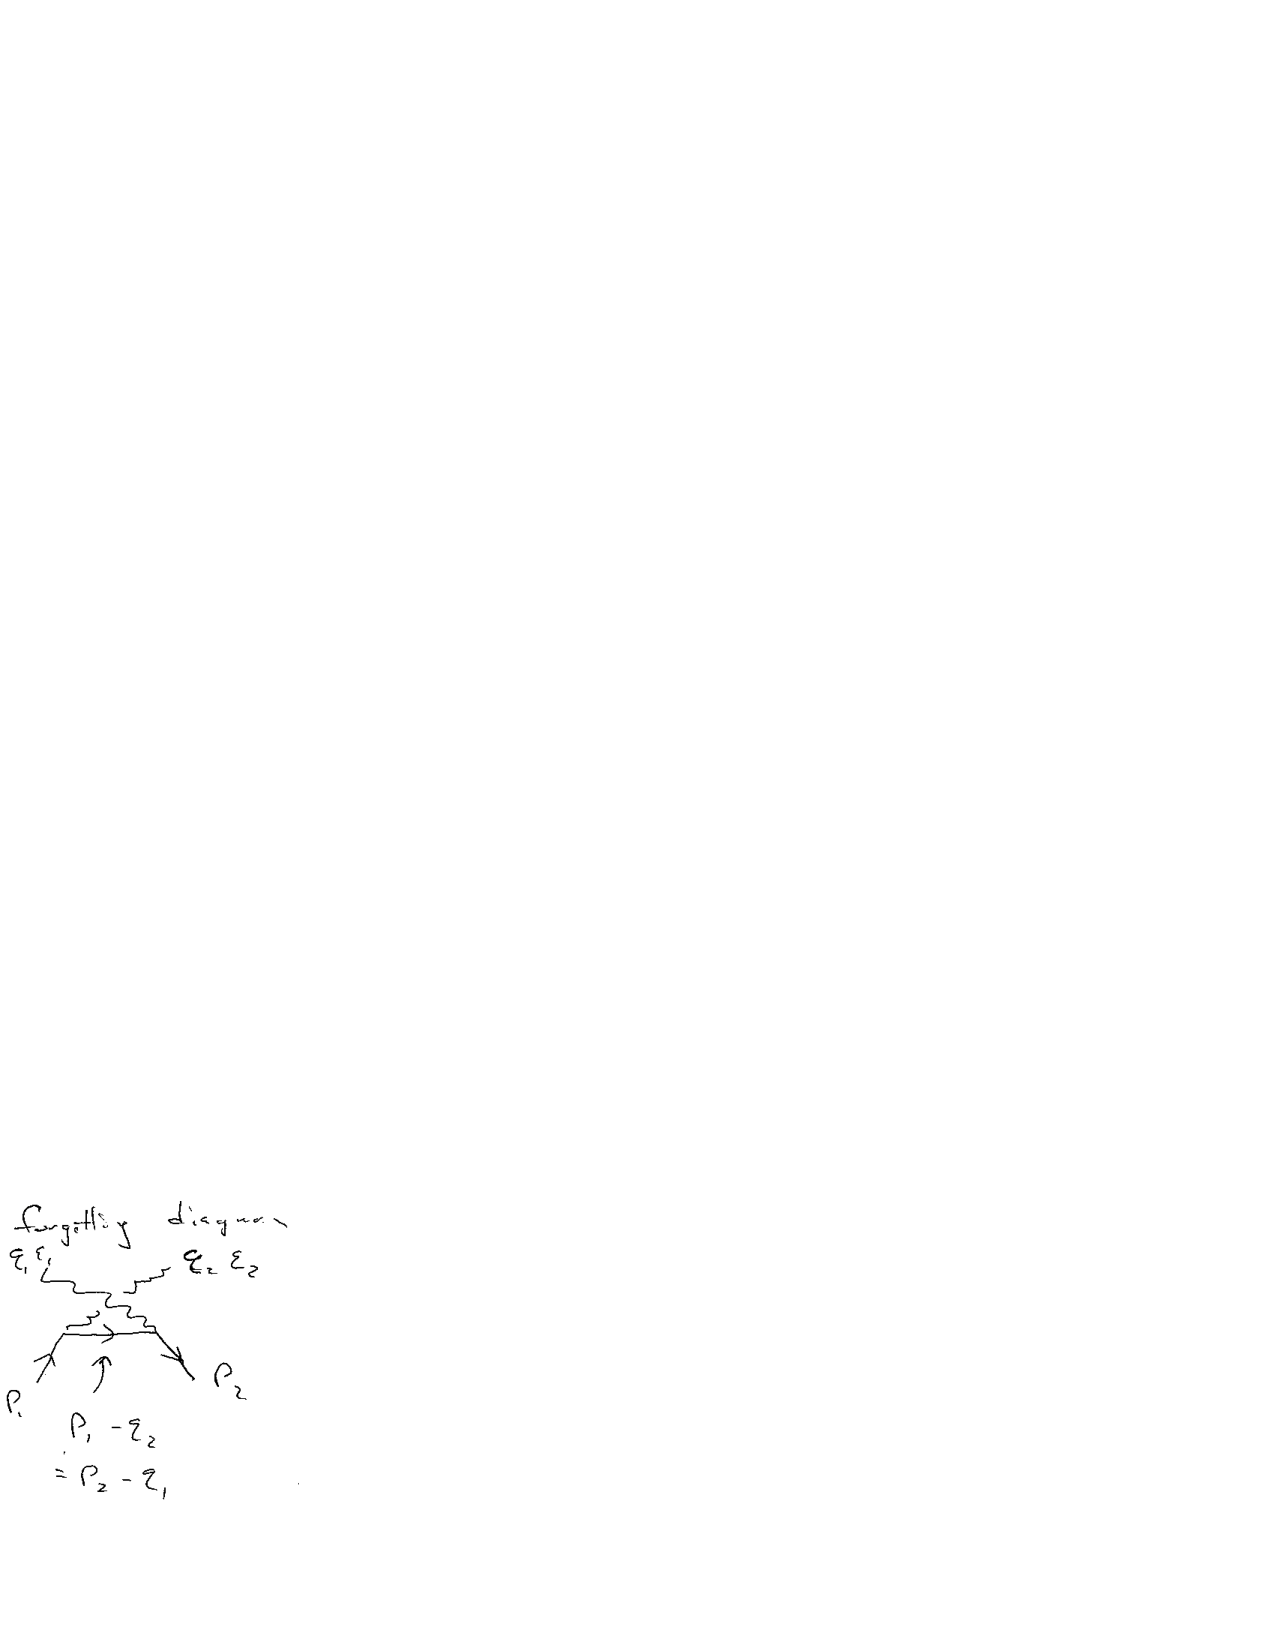
\includegraphics[width=0.5\textwidth]{./comptonScattering2.pdf}
\end{figure}

\bea
&=& (iQ)\epsilon^1_\mu(2 p_2^\mu) \frac{i}{(p_2-q_1)^2 - m^2} (iQ)\epsilon^2_\nu (2p_1^\nu)\\
&=&  \epsilon_1^\mu \epsilon_2^\nu \left( \frac{(-iQ^2) 4 {p_2}_\mu {p_1}_\nu}{-2 p_2\cdot q_1} \right) \underbrace{\sim}_{\textrm{Soft limit $p_1 = p_2$}} \epsilon_1^\mu \epsilon_2^\nu \left( \frac{-(-iQ^2) 2 {p_1}_\mu {p_2}_\nu}{ p_1\cdot q_1} \right) 
\eea

and for this diagram, $ q_1^\mu q_2^\nu M_{\mu\nu} = -(-iQ^2) 2 (p_2\cdot q_2)$

So the sum $M_{\mu\nu}^A + M_{\mu\nu}^B$ is Lorentz Invariant. (Residual non Lorentz Invariant pieces of each diagram cancel)

Very good.

\lineacross 

\clearpage

Now lets do the same thing as before, but with many different possible matter particles. 

$i = 1, ... N_{\textrm{matter}}$

\begin{figure}[h]
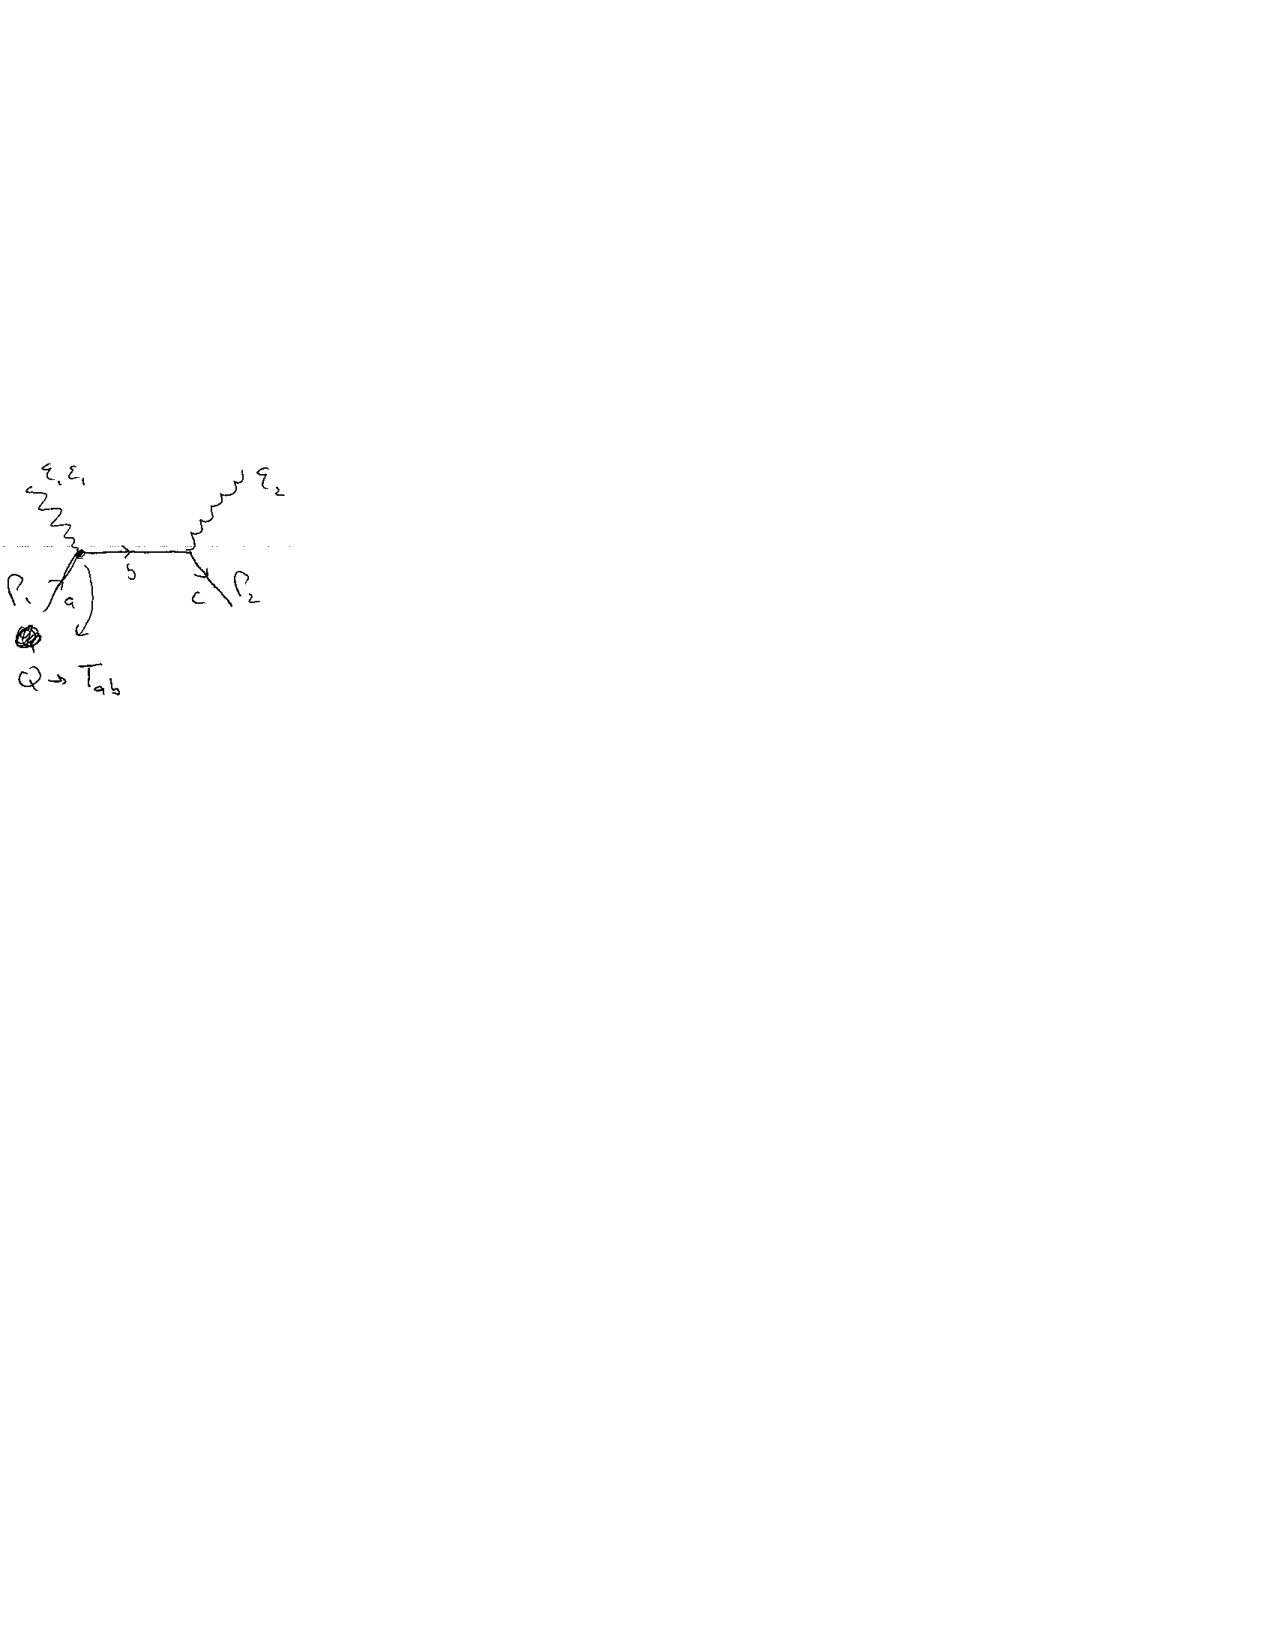
\includegraphics[width=0.5\textwidth]{./comptonScattering3.pdf}
\end{figure}
\bea
&=& (iT_{ab})\epsilon^1_\mu(2 p_1^\mu) \frac{i}{\underbrace{(p_1+q_1)^2 - m^2}_{ m_a^2 +2p_1\cdot q_1 - m_b^2}} (iT_{bc})\epsilon^2_\nu (2p_2^\nu)\\
&=&  \epsilon_1^\mu \epsilon_2^\nu \left( \frac{(-iT_{ab}T_{bc}) 4 {p_1}_\mu {p_2}_\nu}{m_a^2 +2p_1\cdot q_1 - m_b^2} \right) \equiv M^{\mu\nu}_A
\eea

\clearpage

Other diagram
\begin{figure}[h]
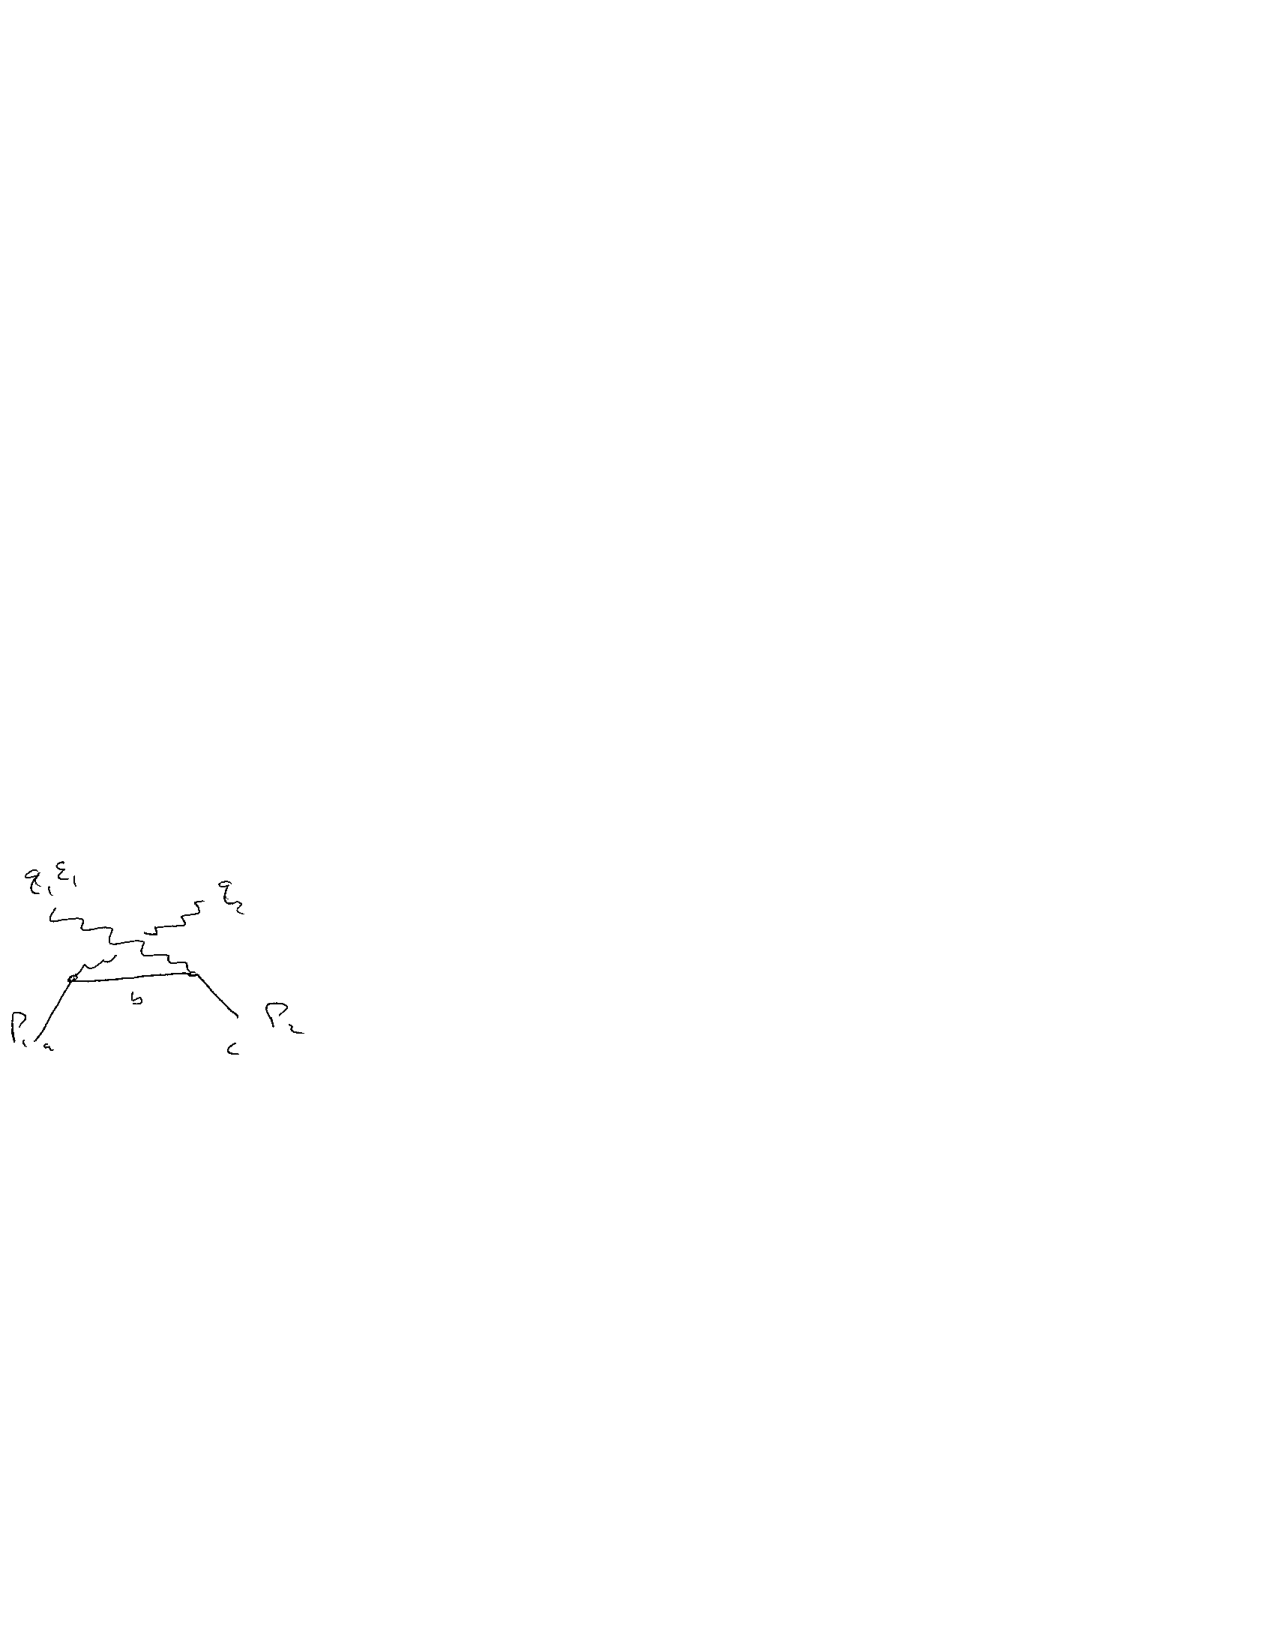
\includegraphics[width=0.5\textwidth]{./comptonScattering4.pdf}
\end{figure}
\bea
&=&  \epsilon_1^\mu \epsilon_2^\nu \left( \frac{(-iT_{ab}T_{bc}) 4 {p_2}_\mu {p_1}_\nu}{m_a^2 - 2p_2\cdot q_1 - m_b^2} \right) \equiv M^{\mu\nu}_B 
\eea

Now, if $m_a = m_b = m_c$ then, $ {q_1}_\mu {q_2}_\nu (M^{\mu\nu}_A + M^{\mu\nu}_B) = 0 $ as above \multiline{$m_a^2 - m_b^2 = 0$ \\ relative - size}

However if $m_a \ne m_b$, in soft limit

$ {q_1}_\mu {q_2}_\nu (M^{\mu\nu}_A + M^{\mu\nu}_B) = -\left[ \frac{(-iT_{ab}T_{bc})4}{m_a^2 - m_b^2}  (2 p_1^\mu p_1^\nu) \right] \ne 0$

{\Large Massless spin-1 particles can only interact with particles of the same mass!}

\lineacross

\clearpage

Now allow many differnt \multiline{matter fields \\ (but same mass!)} and many force carriers ``gluons'' 

$i = 1, ... N_{\textrm{matter}}$

$I = 1, ... N_{\textrm{gluons}}$

\begin{figure}[h]
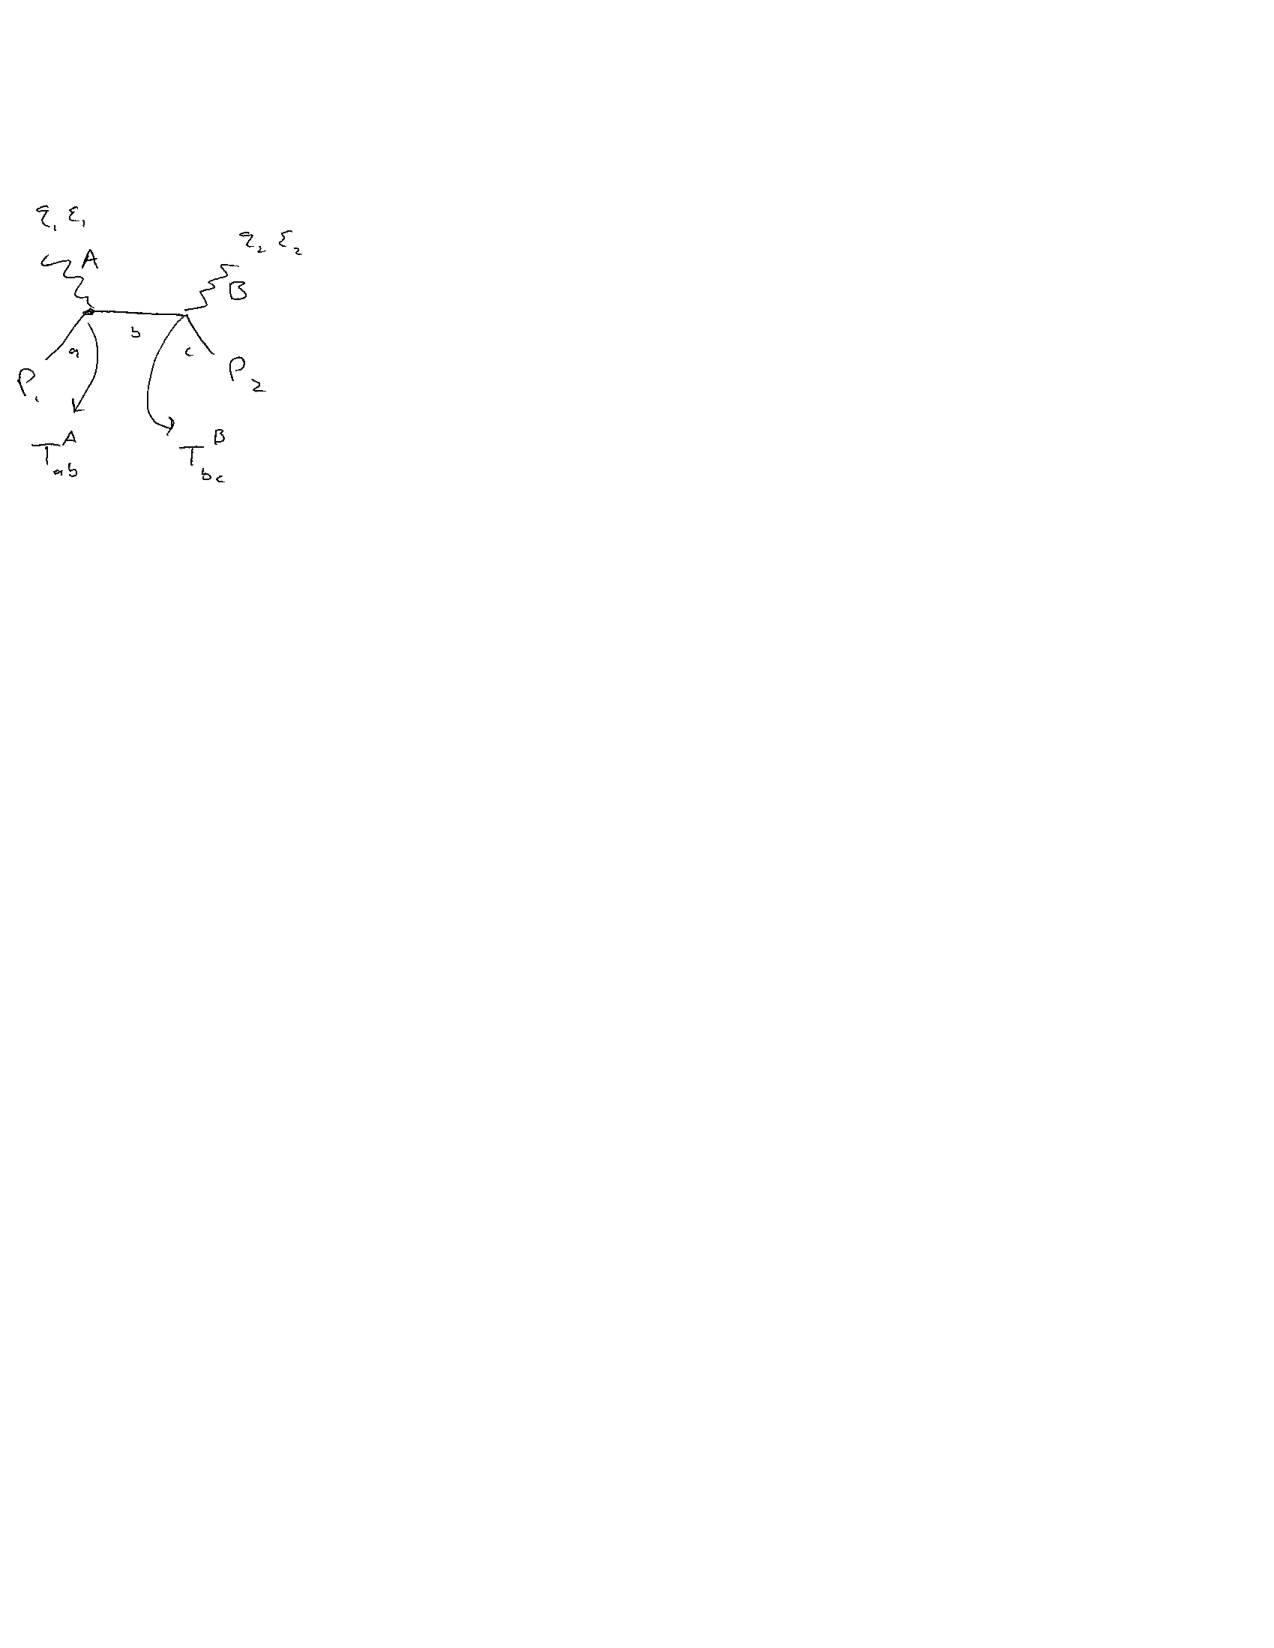
\includegraphics[width=0.3\textwidth]{./comptonScattering5.pdf}
\end{figure}
\bea
&=&  \epsilon_1^\mu \epsilon_2^\nu \left( \frac{(-iT_{ab}^AT_{bc}^B) 4 {p_1}_\mu {p_2}_\nu}{2p_1\cdot q_1 } \right) \equiv M^{\mu\nu}_A
\eea

and 

\begin{figure}[h]
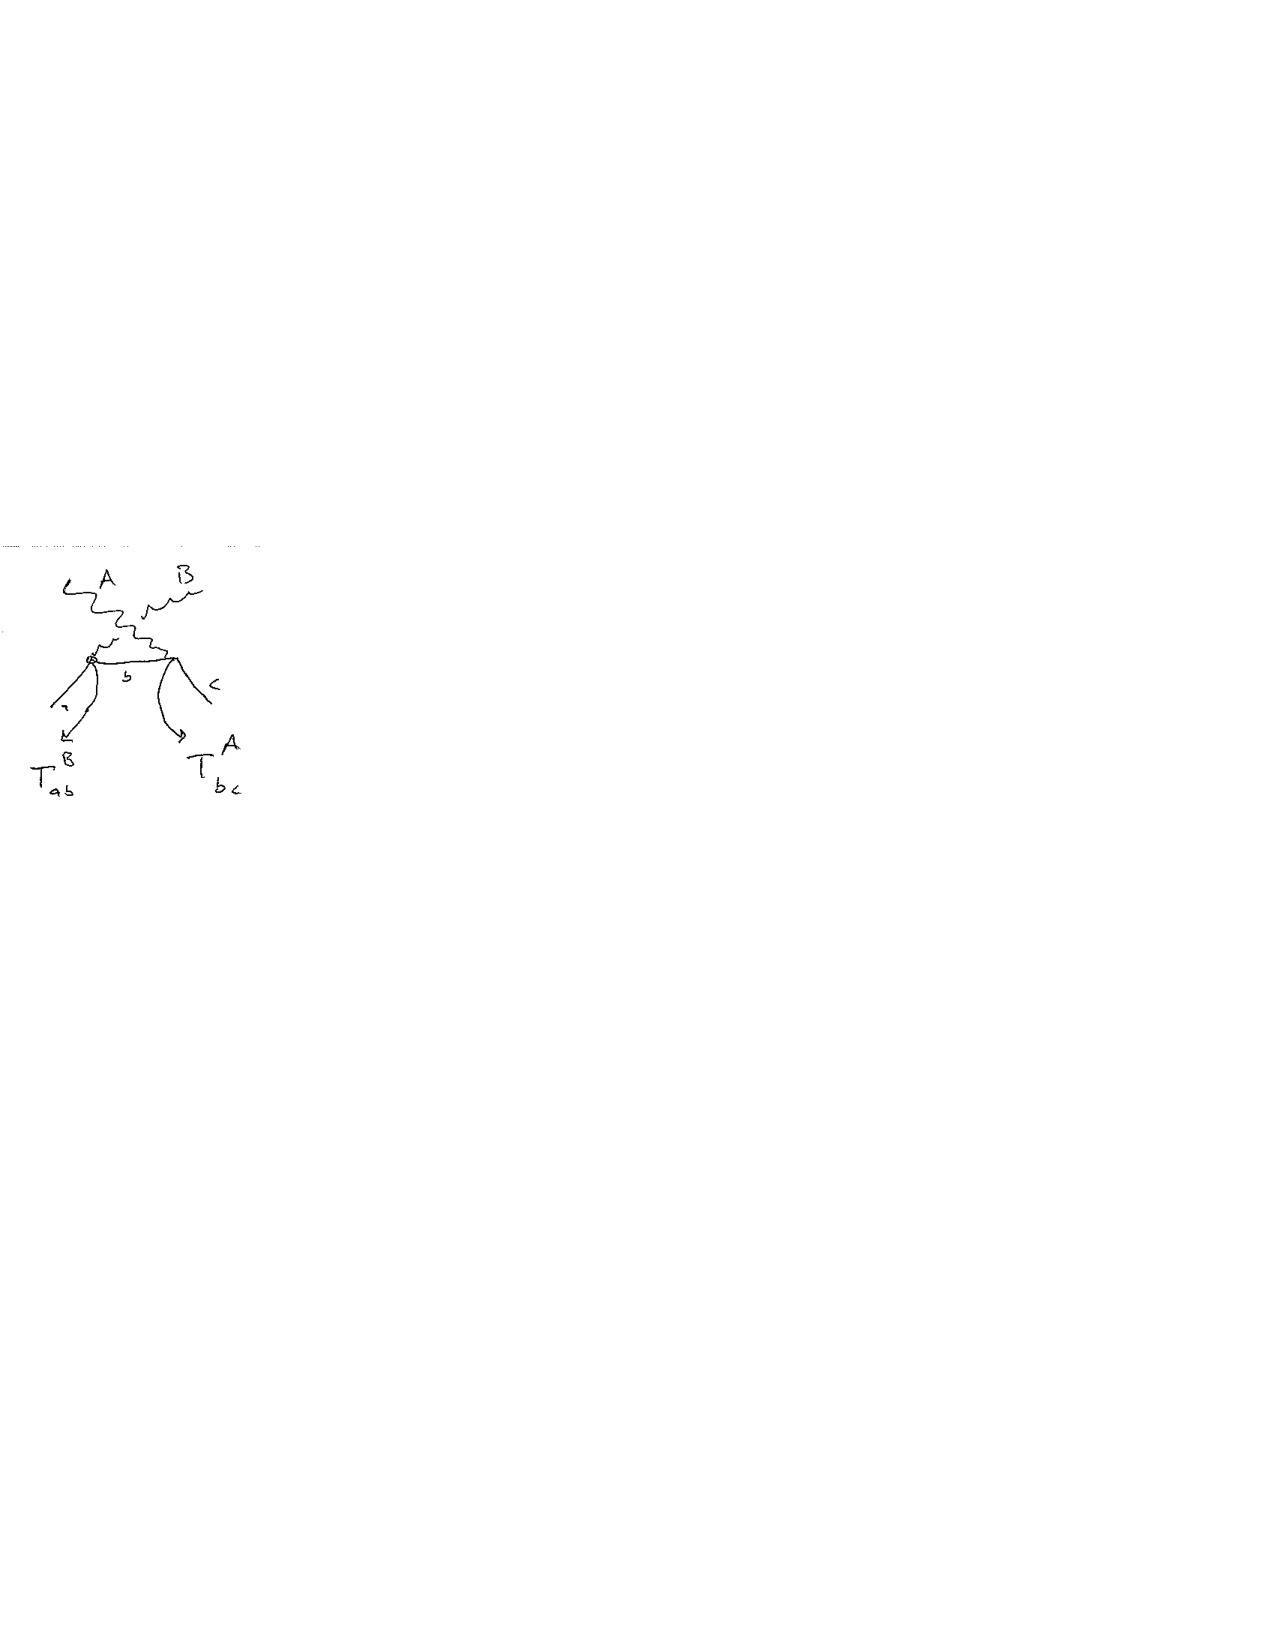
\includegraphics[width=0.3\textwidth]{./comptonScattering6.pdf}
\end{figure}
\bea
&\underbrace{=}_{\textrm{``soft limit''}}&  \epsilon_1^\mu \epsilon_2^\nu \left( \frac{(-iT_{ab}^BT_{bc}^A) 4 {p_1}_\mu {p_2}_\nu}{- 2p_1\cdot q_1 } \right) \equiv M^{\mu\nu}_B
\eea

Now, 

\bea
 {q_1}_\mu {q_2}_\nu (M^{\mu\nu}_A + M^{\mu\nu}_B) &=& 2(-i)(p_2\cdot q_2)(T_{ab}^AT_{bc}^B - T_{ab}^BT_{bc}^A) \\ 
&=& 2(-i)(p_2\cdot q_2) [T^A, T^B]
\eea
$[T^A, T^B]$ not 0 for random Ts. 

In fact 

\begin{figure}[h]
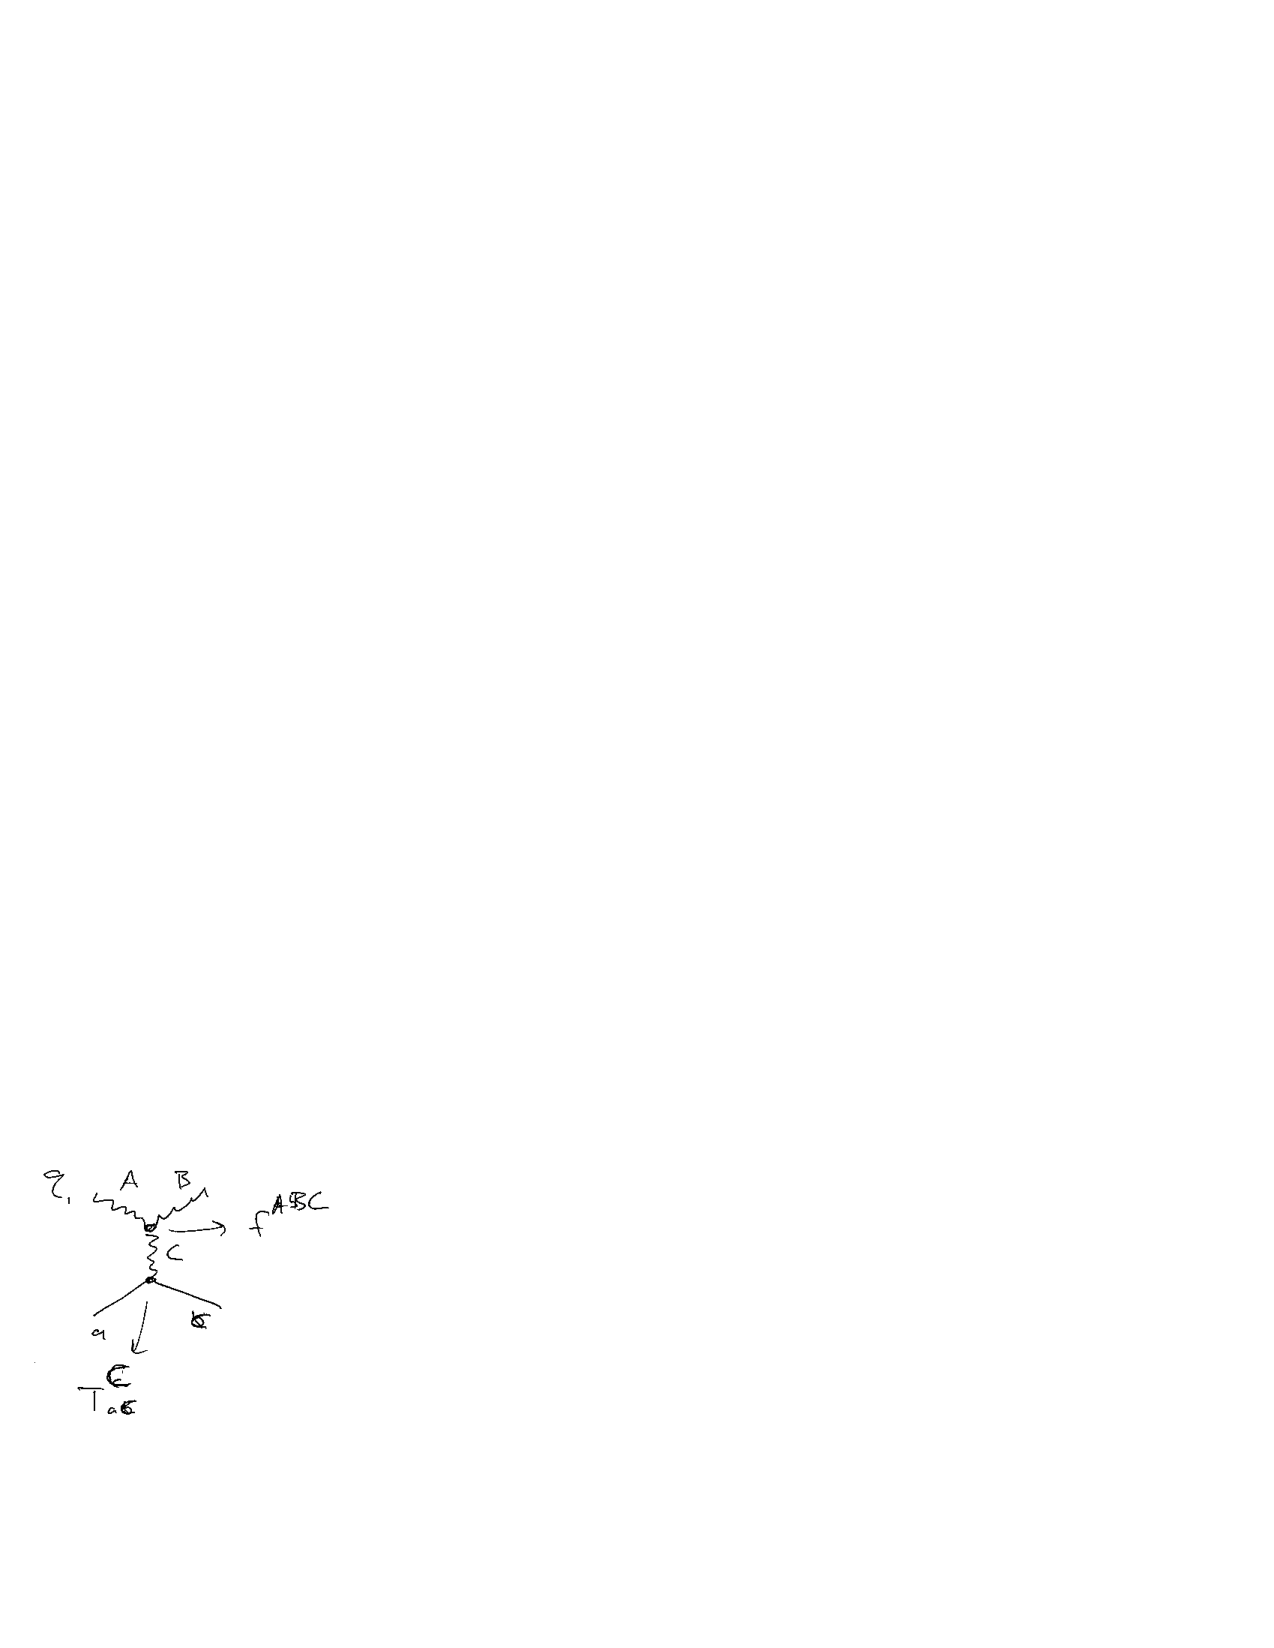
\includegraphics[width=0.3\textwidth]{./comptonScattering7.pdf}
\end{figure}
\be
= + 2i (q\cdot q) i f^{ABC} T_{ac}^C 
\ee

Sum of all three only lorentz invariant if 

\be
[T^A, T^B] = i f^{ABC} T^C
\ee


``gluons'' (or any other group of interacting massless spin-1 particles) must transform as a Lie group ! 

Only question is which group, there are only a finite handful of possibilities


``Yang-Mills'' Interaction. 


}
\end{document}

